\section{Git}

\subsection{Lingo}
\begin{itemize}

    \item origin: default name for your remote repository
    
    \item head: \emph{your} last \emph{commit} on the current branch. Does not yet include non-commited changes. 
        \begin{itemize}
            \item When you switch branches with \inlinecode{git checkout}, the HEAD revision changes to point to the tip of the new
            branch.
            \item When you do a \inlinecode{git pull}, your working directory may contain new stuff, which your head is lagging behind. To see the difference between the working dir and your last commit, do \inlinecode{git diff HEAD}
        \end{itemize}
        
    \item index: The index is a single, large, binary file in baseOfRepo/.git/index, which lists all files in the current branch, their sha1 checksums, time stamps and the file name
    
\end{itemize}



\paragraph{Merging remote changes on master into local master} It can happen that somebody else has been messing with the master before you had a chance to commit your own changes. You will notice this by seeing your \inlinecode{git push} fail. In that case, try to first merge the remote changes into your local copy before pushing again. 
\begin{lstlisting}
git commit // first saving our latest changes
git fetch  // getting remote stuff in remote-tracking-branches. Doesn't change our files yet
git diff master origin/master // compares what you have in master vs. what happened to master remotely
git merge remotes/origin/master
\end{lstlisting}
This will try to merge the upstream changes into yours. If it fails, the conflicting file will contain annotations like these: 
\begin{lstlisting}
<<<<<<< HEAD
print("159 just edited this file")
=======
print("133 just edited this file")
>>>>>>> master
\end{lstlisting}
As you can guess, \inlinecode{<<<<<HEAD} is your code, \inlinecode{===} is a separator, and \inlinecode{>>>> master} is the end of the other guys code. 
Use a texteditor to resolve all conflicts. Eclipse actually has a graphical interpreter for the conflict-tags. Once the resolving is completed, a \inlinecode{git push} and \inlinecode{git commit} will complete the merge.
\begin{lstlisting}
git status // shows that there is still a conflict
git add .
git status // shows that conflict is resolved, but merging still in progress
git commit -m "phew! managed to resolve the conflict!"
git push origin master
\end{lstlisting}



\subsection{Changing origin}
\begin{lstlisting}
git remote -v
git remote set-url origin https://github.com/USERNAME/REPOSITORY.git
\end{lstlisting}


\subsection{Merge vs. rebase}

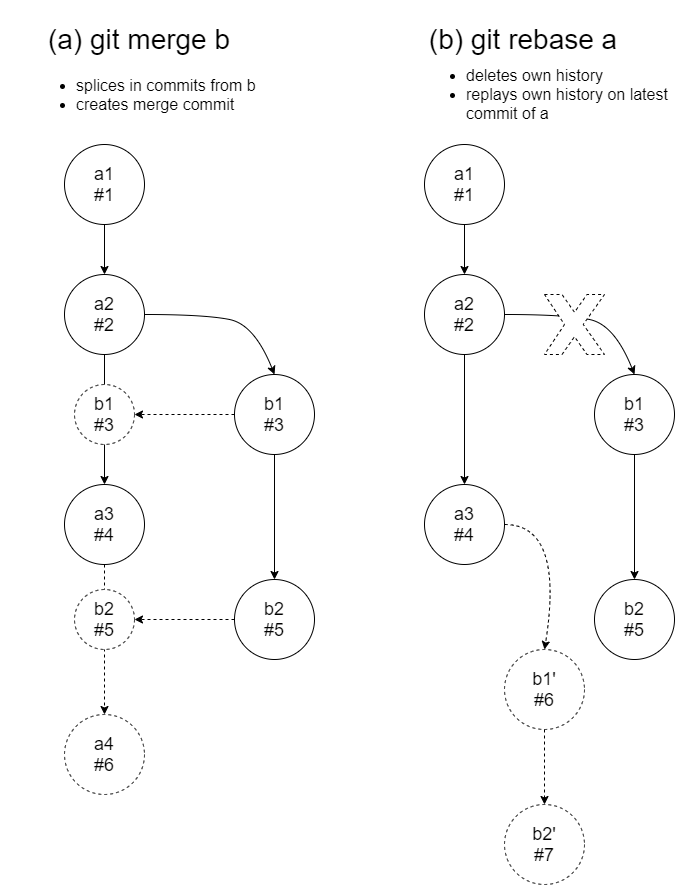
\includegraphics[width=0.8\textwidth]{images/merge_vs_rebase.png}

\paragraph{Reverting and resetting} is best explained in this post: \inlinecode{https://stackoverflow.com/questions/4114095/how-to-revert-git-repository-to-a-previous-commit}. Basically, we have these options: 

\begin{itemize}
    \item \inlinecode{git revert <lastGoodCommitHash>..HEAD} will execute the inverse of all the operations and commit them as a new commit. This way, the old history stays intact.
    \item \inlinecode{git reset <lastGoodCommitHash>} will un-stage all the commits from \inlinecode{<firstBadCommitHash>..HEAD}. This way, you're rewriting history, which is really only good if you're working alone on a repo.
\end{itemize}


\subsection{Moving through history quickly}
\begin{lstlisting}[language=bash]
# checkout prev (older) revision
git_prev() {
    git checkout HEAD~
}

# checkout next (newer) commit
git_next() {
    BRANCH=`git show-ref | grep $(git show-ref -s -- HEAD) | sed 's|.*/\(.*\)|\1|' | grep -v HEAD | sort | uniq`
    HASH=`git rev-parse $BRANCH`
    PREV=`git rev-list --topo-order HEAD..$HASH | tail -1`
    git checkout $PREV
}
\end{lstlisting}

\subsection{Creating your own repository}
Basically, any git folder can be used as a repository. But you still need to do some work to expose that folder over the web. The easiest way to work is certainly over gitlab. For alternative means if you don't have a hoster, this site lists a few of the possibilities: \inlinecode{http://www.jedi.be/blog/2009/05/06/8-ways-to-share-your-git-repository/}.
